\section{Zielsetzung}
In diesem Versuch sollen mithilfe der Tomographie mit Gamma-Strahlung verschiedene Würfel auf ihre Zusammensetzung untersucht werden.
Der Fokus liegt dabei auf dem Verständnis von Tomographie als bildgebendes Verfahren und der Funktionsweise eines Szintillationsdetektors.

\section{Theorie}
\label{sec:Theorie}

\subsection{Tomographie}
Die Tomographie ist ein bildgebendes Verfahren.
Wird ein Objekt bestrahlt, so entstehen zweidimensionale Bildschnitte, welche nach Überlagerung den ganzen Körper darstellen können.
Trifft Strahlung auf Materie, wird diese durch Wechselwirkungen abgeschwächt.
Dabei ergibt sich für die gemessene Zählrate $R$ folgender Zusammenhang:
\begin{equation*}
    R = R_0 \cdot \exp{(- \sum_{i} \mu_i d_i)} \, .
\end{equation*}
$R_0$ beschreibt die Eingangszählrate, $\mu_i$ den Absorptionskoeffizienten und $d_i$ die zurückgelegte Strecke nach Strahlrichtung $i$.
Dabei wird von stückweisen konstanten Absorptionskoeffizienten ausgegagngen. 
Sind Eingangs- und Ausgangszählrate bekannt, kann durch Logarithmieren ein Ausdruck für den Absorptionskoeffizienten aufgestellt werden:
\begin{equation}
    \sum_{i} \mu_i d_i = \ln\left(\frac{R_0}{R}\right) \, .
    \label{eqn:SUMME}
\end{equation}
Durch die 12 verschiedenen Projektionen in der Messung und die unbekannte Zusammensetzung des zu messenden Würfels 
entsteht ein lineares Gleichungssystem, sodass \eqref{eqn:SUMME} in Matrixschreibweise dargestellt werden kann:
\begin{equation}
    A \vec{\mu} = \vec{I} \, ,
    \label{eqn:matrix}
\end{equation}
wobei $\vec{I}$ ein Vektor mit den zwölf Einträgen $\vec{I}_i = \ln\left(\frac{R_0}{R_i}\right)$ mit der gemessenen Zählrate $R_i$ in der Projektion $i$ ist.
Die Matrix A die verschiedenen Strecken, die bei einer Projektion durch ein Material von der Strahlung durchlaufen werden.
% Das entstandene LGS soll überbestimmt sein.
Die Matrix $A$ sollte nicht singulär sein, damit die Werte für die Absorptionskoeffizienten mit dem Verfahren für die kleinsten Quadrate gefittet werden können.
Es ergibt sich folgender Ausdruck für den Absorptionskoeffizienten $\mu$:
\begin{equation*}
    \vec{\mu} = \left( A^\top \cdot A \right)^{-1} \cdot A^\top \vec{I}
\end{equation*}

\subsection{Projektionen}
Um keine singuläre Matrix A zu erhalten, werden die in \autoref{fig:Projektionen} gezeigten Projektionen für die Messungen verwendet.
Insgesamt gibt es 12 Projektionsrichtungen.

\begin{figure}[H]
    \centering
    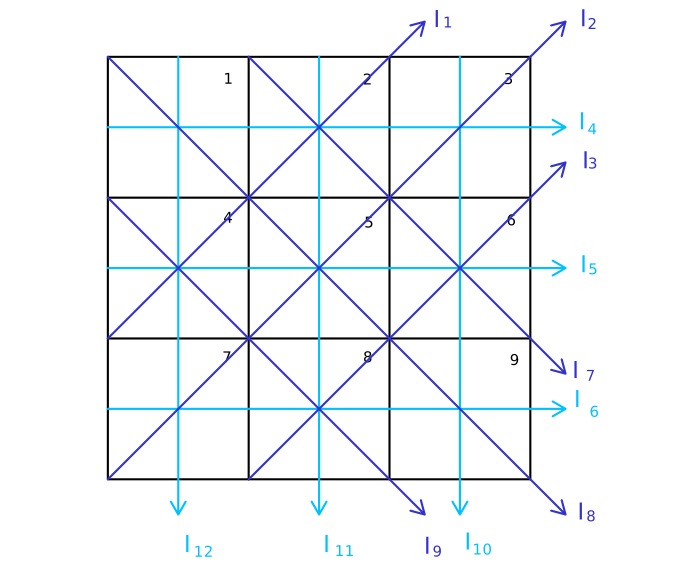
\includegraphics[width=\textwidth]{bilder/projektionen.png}
    \caption{Schematischer Aufbau der verwendeten Projektionen.Die Benennung der kleineren Würfel erfolgt auch nach dieser Abbildung, wobei die Zahl auf dem Würfel aufrecht zu lesen ist}
    \label{fig:Projektionen}
\end{figure}

\noindent
Die Matrix $A$ nimmt somit die folgende Form an, wenn $d$ die Seitenlänge der kleineren Würfel ist:
\begin{equation}
    A = d \begin{pmatrix} 
        0       & \sqrt{2} & 0      & \sqrt{2}  & 0         & 0         & 0         & 0         & 0         \\
        0       & 0        &\sqrt{2}& 0         &\sqrt{2}   & 0         &\sqrt{2}   & 0         & 0         \\
        0       & 0        & 0      & 0         & 0         &\sqrt{2}   & 0         & \sqrt{2}  & 0         \\
        1       & 1        & 1      & 0         & 0         & 0         & 0         & 0         & 0         \\
        0       & 0        & 0      & 1         & 1         & 1         & 0         & 0         & 0         \\
        0       & 0        & 0      & 0         & 0         & 0         & 1         & 1         & 1         \\
        0       & \sqrt{2} & 0      & 0         & 0         & \sqrt{2}  & 0         & 0         & 0         \\
        \sqrt{2}& 0        & 0      & 0         & \sqrt{2}  & 0         & 0         & 0         & \sqrt{2}  \\
        0       & 0        & 0      & \sqrt{2}  & 0         & 0         & 0         & \sqrt{2}  & 0         \\
        0       & 0        & 1      & 0         & 0         & 1         & 0         & 0         & 1         \\
        0       & 1        & 0      & 0         & 1         & 0         & 0         & 1         & 0         \\
        1       & 0        & 0      & 1         & 0         & 0         & 1         & 0         & 0         
    \end{pmatrix}
    \label{eqn:A}
\end{equation}

\subsection{Absorptionsphänomene}
Da Gamma-Strahlung verwendet wird, wird im Folgenden auf die Hauptwechselwirkungen eingegangen.
Die drei wichtigsten Effekte, die bei Photon-Materie Wechselwirkungen auftreten, sind Photoeffekt, Comptoneffekt und Paarbildung.
\begin{itemize}
    \item   Photoeffekt: Wenn ein Photon mindestens eine Energie hat, die so groß ist wie die Bindungsenergie eines Elektrons, dann kann das Elektron durch Aufnahme der Photonenenergie das Atom verlassen.
    
    \item   Comptoneffekt: Dieser Effekt beschreibt einen elastischen Stoß zwischen Photon und Elektron.
            Das Photon wird an einem Elektron gestreut und gibt dabei einen Teil seiner Energie ab.
            Es hat nach dem Stoß eine andere Wellenlänge. Wichtig ist, dass nach dem Stoß das Photon weiter existiert.
    
    \item   Paarbildung: Wenn die Energie eines Photons die Energie eines Elektron-Positron Paares entspricht, kann sich dieses Photon in diese beiden Teilchen aufteilen.
            Dazu muss es auch in der Nähe des Atomkerns sein, welches als Stoßpartner fungiert. 
    
\end{itemize}

\noindent
In diesem Versuch sind die beobachtbaren Effekte der Compton und Photoeffekt.
Da die Energie der Gamma-Strahlung bei $\SI{662}{\kilo\electronvolt}$ \cite{LEIFI} liegt, kommt es zu keiner Paarbildung.
Die dafür benötigte Energie muss bei $2 \cdot \SI{511}{\kilo\electronvolt}$ liegen.

\subsection{Gammaspektrum von $\ce{^{137}Cs}$}
In \autoref{fig:LEIFI_CS_Spektrum} ist das Spektrum von $\ce{^{137}Cs}$ zu sehen.
Der Photopeak bzw. der Full Energy Peak ist deutlich bei einer Energie von $\SI{662}{\kilo\electronvolt}$ zu erkennen. 
Die Comptonkante befindet sich bei einer Energie von ungefähr $\SI{460}{\kilo\electronvolt}$. Dies 
entspricht einem Streuwinkel von $\theta = \SI{180}{\degree}$. Der Rückstreupeak, der auch gekennzeichnet ist, 
entspricht Comptonphotonen, die nach Comptonstreuung mit z.B. der Rückwand der Präparathalterung, in den Szintillationsdetektor kommen.  

\begin{figure}[H]
    \centering
    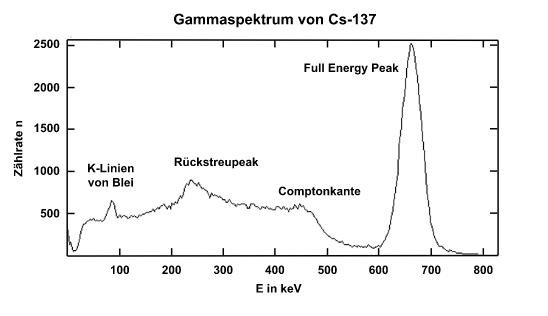
\includegraphics[width=\textwidth]{bilder/LEIFI_Cs_Spektrum.png}
    \caption{Gammaspektrum von $\ce{^{137}Cs}$.\cite{LEIFI}}
    \label{fig:LEIFI_CS_Spektrum}
\end{figure}


% \subsection{Absorptionskoeffiziente}
% Da die Untersuchung der Würfel bzw. die Materialbestimmung über die Ermittlung der Absorptionskoeffizienten läuft, werden in \autoref{tab:lit_theo} die Koeffizienten der möglichen Materialien aufgenommen.
% Die ermittelten Absorptionskoeffizienten werden mit den Litaraturwerten verglichen um so auf das Material im jeweiligen Würfel zu schließen.
% 
% \begin{table}
    % \centering
    % \caption{Die Literaturwerte des Massenschwächungskoeffizienten $\sigma$ , der Stoffdichte $\rho$ und dem Absorptionskoeffizienten $\mu$ der mögliche Materialien.}
    % \label{tab:lit_theo}
    % \begin{tabular}{c S[table-format=2.3] S[table-format=2.2] S[table-format=1.3]}
        % \toprule
        % {Stoff} & {$ \sigma \mathbin{/}  \left(\SI{e-2}{\centi\metre\squared\per\gram}\right)$\cite{massenbumms}} & {$\rho \mathbin{/}  \left(\si{\gram\per\centi\metre\cubic}\right)$\cite{dichten}} & {$\mu \mathbin{/} \left( \si{\per\centi\metre\cubic}\right)$} \\
        % \midrule
        % Aluminium & 7.802   & 2.7   & 0.211 \\
        % Blei      & 12.48   & 11.34 & 1.415 \\
        % Eisen     & 7.704   & 7.87  & 0.606 \\
        % Messing   & 7.651   & 8.4   & 0.642 \\
        % Delrin    & 8.6     & 1.42  & 0.121 \\
        % \bottomrule
    % \end{tabular}
% \end{table}